\Chapter{Animáció}
\label{Chap:animacio}

%A csontváz kezelésének és számítógépen való ábrázolásának bemutatása
%
%- Kulcsképkocka animáció
%- Csontváz alapú animáció
%- Blender-es animációs formátum
%- Egyszerűbb görbék bemutatása, amelyeket animációkhoz használnak (interpolációs módszerek)
%
%A mesterséges intelligencia és az evolúciós algoritmusok szerepe a probléma megoldásában
%
%- Megnézni azt a cikket, amihez az animációs videó készült.
%- Felvetni néhány módszert, például ANN vagy evolúciós algoritmus. (Itt még nem kell majd %implementálni, egyelőre csak legyen összegyűjtve.)

A fejezet a játékokban alkalmazott animációs módszereket módszereket, illetve azok megvalósítási módját mutatja be.

\section{Kulcsképkocka alapú animáció}

Kulcsképkocka alapú mozgatást több területen használnak, például filmek készítésénél vagy játékok fejlesztésénél. Bármilyen célra is használjuk, az elv nem változik. Meg kell adnunk olyan pontokat, amelyeket szeretnénk ha az adott tárgy, vagy objektum áthaladna. Ezzel egy előre meghatározott mozgási útvonalat adunk meg. Az egyszerűbb animációknál egy alapállapot és egy végállapot van megadva, ilyen lehet egy redőny leengedése és felhúzása, ajtó vagy kapu kinyitása, becsukása. Ilyen jellegű, alap szintű animációknál, például ha egy redőnyt le akarunk engedni, annyi a dolgunk hogy megadjuk a kezdő és végpontot, majd idő paraméter szerint interpolálni. Ahogy az \aref{fig:keyframe} ábrán látható, ez a kulcsképkockák közötti mozgást eredményezi.

\begin{figure}[h]
\centering
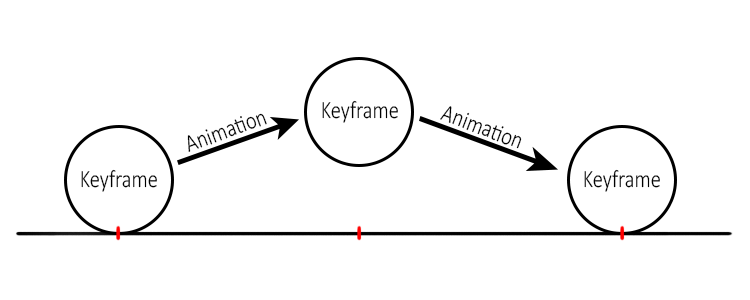
\includegraphics[scale=0.5]{kepek/keyframe_anim.png}
\caption{Kulcsképkocka alapú animáció}
\label{fig:keyframe}
\end{figure}

A vertex alapú animációt a 3D játékfejlesztésben karakterek mozgatásához a 2000-es évek elejéig használták. Megvalósítása egyszerűbb, viszont sok memóriát igényel a tárolása, és nem eredményez olyan természetes mozgást általában, mint a csontváz alapú animáció. Ezt a technológiát többek között a Quake 1, 2 és 3 alkalmazta.

\subsection{Az md2-es formátum}

Az md2-es modelltárolási formátumot az \textit{idSoftware} fejlesztette ki 1997-ben a Quake 2 nevű játékához. A formátum kulcsképkocka animációk tárolására alkalmas. Tartalmazza az adott modell geometriáit, és a képkockánkénti animációkat. A fájl adatai olyan struktúrában helyezkednek el, hogy könnyedén kirajzoltatható legyen a \texttt{GL\_TRIANGLE\_FAN} és \texttt{GL\_TRIANGLE\_STRIP} OpenGL függvényekkel. A formátum két fő részből áll: fejlécből és adatrészből. A fájl nem tartalmazza a modellek textúráját.

A fejléc egy struktúra, amely a fájl elején kezdődik, és tartalmazza az összes, feldolgozás szempontjából lényeges információt a fájl egészéről. Ilyen például a textúra szélessége, magassága, egy képkocka mérete, képkockák száma.

Az animáláshoz ezt a módszert választottam, mert viszonylag egyszerűen implementálható. Egyetlen jelentős hátrányaként az hozható fel, hogy aránylag nagy a tárigénye más formátumokkal összehasonlítva.

\section{Csontváz alapú animáció}

A legtöbb mai játék ezt a módszert alkalmazza karakterek mozgatásához. Az alapötlete az, hogy a mozgatható részeket hierarchiába szervezi. Az élőlények felépítése általában olyan, hogy ezzel a fajta animálási móddal egyszerűen modellezhetők. 

A csontváz alapú animáció kapcsolódási pontokból (\textit{joint}-okból) építkezik. Ember esetén például a kézfej kapcsolatban van az alkarral, az alkar a felkarral, ami pedig a test többi részével. Minden hajlási pont egy új kapcsolódási pontot jelent. Tehát a az ember felkarját megmozdítjuk, mozdul vele a kezének a többi része is. Ezt szemlélteti \aref{fig:skeletal}. ábra.

\begin{figure}[h]
\centering
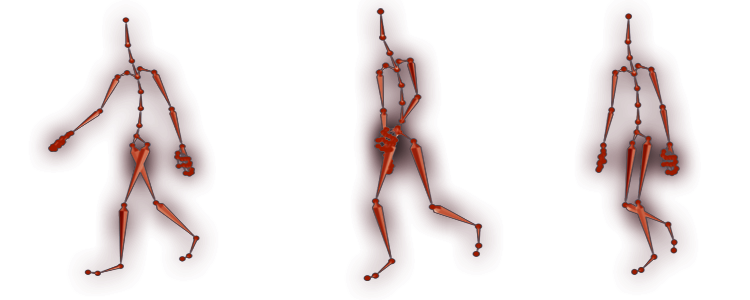
\includegraphics[scale=0.5]{kepek/skeletal_anim.png}
\caption[]{Testrészek hierarchikus kapcsolódási pontjai emberen\footnotemark}
\label{fig:skeletal}
\end{figure}

\footnotetext{forrás: https://www.openflipper.org/media/plugin\_images/skeletalAnimation.png}

Szerencsére a módszer nem csak élőlények modellezésére alkalmazható hatékonyak. A naprendszerünk szintén modellezhető ilyen módon. Vannak a naprendszerünk bolygói, amelyek a tengelyük, és a központi csillag, a Nap körül is forognak.

Előnye, hogy könnyen létre lehet így hozni dinamikus animációkat, mivel az összes karakter csontjait lehet forgatni, mozgatni, továbbá megkönnyíti a bonyolultabb animációk elkészítését. Hátránya viszont, hogy komplexebbek, így több processzoridőt igényelnek.

\subsection{Csontváz alapú animációhoz támogató fájlformátum}

A csontváz alapú animációkat tároló formátumok általában két részből állnak. Az egyik a geometriát, a másik pedig a csontvázat és a kapcsolódási pontokat tartalmazza. 

% TODO: Ez itt pontosan mi lenne?

Ha két csont tartozik minden vertex-hez, a felépítés a következőképp alakul:
\begin{itemize}
\item A vertex x,y,z koordinátája
\item Normálvektor x,y,z iránya
\item Textúra u,v koordinátái
\item Indexek (index1, index2) a csont/eltolás mátrix tömbjéhez (2 csont esetében)
\item Weight1, weight2, ami az egyes csontok átfedési tényezője (2 csont esetében)
\end{itemize}

\section{Interpolációs módszerek}

% Interpoláció: https://hu.wikipedia.org/wiki/Interpol%C3%A1ci%C3%B3#Lagrange-interpol.C3.A1ci.C3.B3

Animációkészítés során többféle interpolációt használhatunk, ami azt jelenti, hogy ismert értékek alapján, a közbülső pontokra, vagyis nem ismert értékekre adunk közelítést.

Különféle interpolációs módszerek vannak. A választás közülük nyilván attól függ, hogy pontosan mit szeretnénk megvalósítani. Egyszerűbb esetekben még megfelelő a lineáris interpoláció, viszont általában túlságosan szögletes mozgást eredményez, ezért valamilyen simább görbével való útvonal közelítést érdemes használni.

\subsection{Lineáris interpoláció}

Ez a legegyszerűbb interpolációs módszer, minden pontot egy egyenessel kötünk össze. Nem összetett mozgásoknál ez megfelelő lehet, viszont ha több mozgás követi egymást rögtön, akkor darabos. Minden előre meghatározott pont, amit érinteni kell egy törést jelent, így komplexebb, sima mozgásokhoz nem alkalmas, ez látható \aref{fig:linear}. ábrán.

\begin{figure}[h]
\centering
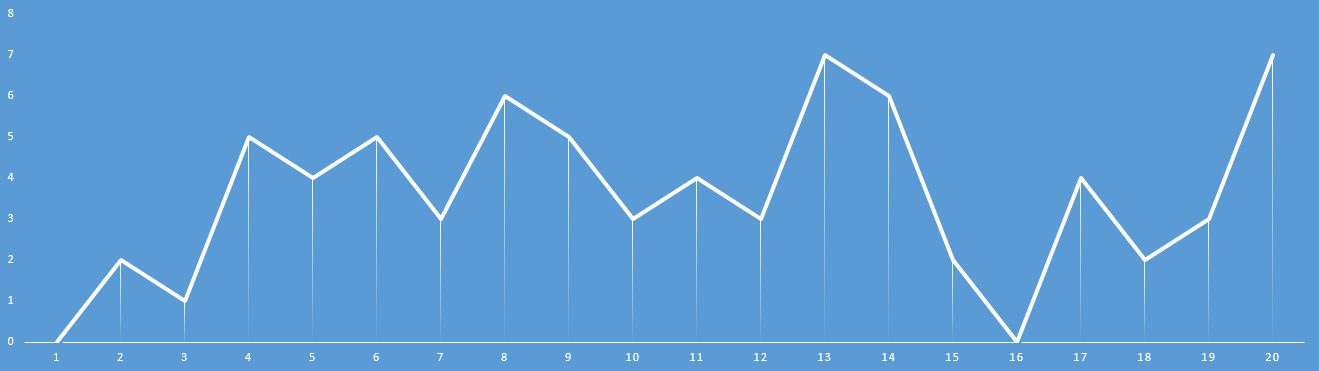
\includegraphics[scale=0.43]{kepek/linear_interpol.png}
\caption{Lineáris interpoláció}
\label{fig:linear}
\end{figure}

\subsection{Lagrange-interpoláció}

Komplexebb animációknál, mint például egy élőlény mozgása, ha nem szeretnénk darabos animációt, akkor alkalmazhatjuk a Lagrange-interpoláció módszerét. ez egy lehetséges megoldás. Mivel a függvény sima, deriváltja folyontos, sokkal életszerűbb megközelítést lehet elérni vele, ez látható \aref{fig:lagrange}-es ábrán. 

% TODO: Meg kellene nézni, hogy valóban mennyire alkalmas mozgás animációjához!

\begin{figure}[h]
\centering
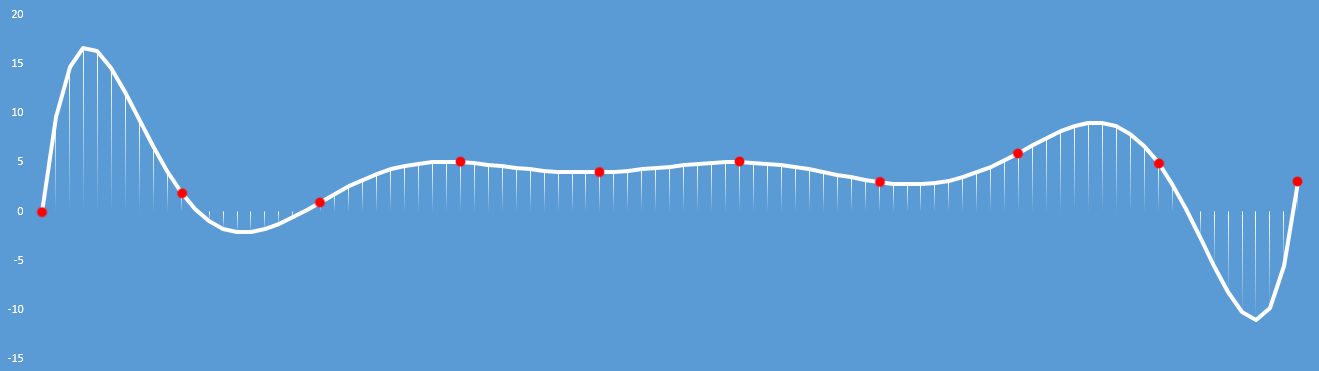
\includegraphics[scale=0.43]{kepek/non_linear_interpol.png}
\caption{Lagrange-interpoláció}
\label{fig:lagrange}
\end{figure}

\subsubsection{Megvalósítás}

A felhasználónak lehetősége van beírni egy x értéket, amelyhez a program kiszámolja az y koordinátát Lagrange-interpolációval. Ez a program azért készült, hogy bemutassa, hogyan működik ez a fajta interpolálás.
Adott két tömb, amelyek tartalmazzák a függvény megadott pontjainak x és y értékeit. A num a tömbök elemeinek számát, az input pedig a bevitt értéket takarja.

\begin{algorithm}[H]
 \KwData{x[]; y[]; num; input; s; t; eredmeny\;}
 \KwResult{Adott x-hez tartozó y koordináta}
\For{i := 0; i < num; i++}{
	s := 1, t := 1\;
	\For{j := 0; j < num; j++}{	
	\If{j != i}{
   		s := s * (input - x[j]);\\
		t := t * (x[i] - x[j])\;
   		}
	}
	eredmeny := eredmeny + ((s / t) * y[i])\;
 }
 \caption{Lagrange-interpoláció implementálása}
\end{algorithm} 

\begin{figure}[h]
\centering
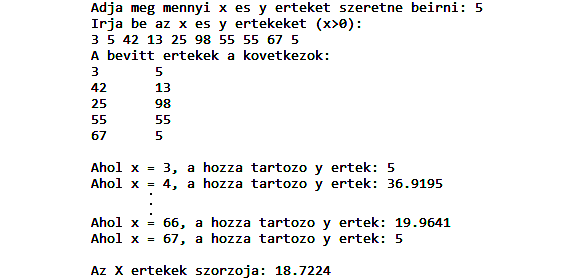
\includegraphics[scale=0.9]{kepek/lagrange_imp.png}
\caption{Lagrange-interpolációs demó}
\label{fig:lagrange_imp}
\end{figure}

